%!TeX log
\documentclass[11pt]{report}

\usepackage{float}
\usepackage{booktabs}
\usepackage[many]{tcolorbox}
\usepackage{tikz}
\usepackage[linewidth=1pt]{mdframed}
\usepackage[utf8]{inputenc}
\usepackage[T1]{fontenc}
\usepackage[english]{babel}
\usepackage{xcolor,colortbl}
\usepackage{geometry}
\usepackage{array,ragged2e}
\usepackage{makecell}
\usepackage{tocloft}
\usepackage[scaled=0.85]{beramono}

\usetikzlibrary{fit, positioning, shapes.arrows}

\geometry{
    a4paper,
    hmargin=12.7mm,
    vmargin=19.35mm,
    head=0ex,
    foot=0ex,
}

\title{Extensible Homebrew Computer \\ System Architecture Specification}
\author{Minsu Kwon (kms1212)}
\date{\today}

\begin{document}

\makeatletter
\begin{titlepage}
    \thispagestyle{empty}
    \vspace*{\fill}
    \hspace*{\fill}
    \begin{tabular}[c]{@{}p{0.8\textwidth}@{}}
        \raggedleft\Huge\textbf{\@title}\\[1em]
        \raggedleft\LARGE\@author\\[2em]
    \end{tabular}
    \vspace*{\fill}
    \clearpage
\end{titlepage}
\makeatother

\newpage
\vspace*{\fill}
\section*{License Information}

\begin{flushleft}
All files in this repository excluding documents which specifies any other
license in its header or “LICENSE” file of its parent directory follow BSD
license, except for the  that the font data of documentations using template
which is used in this documentation:  The contents of this repository
do not warrant its proper operation, and does not warrant its correct
documentation. Reading this document, it is recommended to check its desired
operation from code or binary files on your own.
\end{flushleft}

\paragraph{Trademarks}

\begin{itemize}
    \item IBM-PC is a registered trademark of International Business Corporation.
    \item Macintosh is a trademark of Apple Inc.
    \item UNIX is a registered trademark of AT\&T.
    \item FLEX, MAX, and Altera is a registered trademark of Altera Corp.\ acquired by Intel Corp.
    \item AVR is a registered trademark of Atmel Corp.\ acquired by Microchip Technology Inc.
\end{itemize}

\begin{center}
\begin{tcolorbox}[enhanced jigsaw, colback=white, colframe=black, boxrule=0.75pt, width=0.8\textwidth, arc=0pt, outer arc=0pt, drop shadow=black]
    BSD 3-Clause ``New'' or ``Revised'' License \\
    Copyright 2024 Minsu Kwon \\
    Redistribution and use in source and binary forms, with or without modification, are permitted provided that the following conditions are met:

    \begin{enumerate}
        \item Redistributions of source code must retain the above copyright notice, this list of conditions and the following disclaimer.
        \item Redistributions in binary form must reproduce the above copyright notice, this list of conditions and the following disclaimer in the documentation and/or other materials provided with the distribution.
        \item Neither the name of the copyright holder nor the names of its contributors may be used to endorse or promote products derived from this software without specific prior written permission.
    \end{enumerate}

    THIS SOFTWARE IS PROVIDED BY THE COPYRIGHT HOLDERS AND CONTRIBUTORS ``AS IS'' AND ANY EXPRESS OR IMPLIED WARRANTIES, INCLUDING, BUT NOT LIMITED TO, THE IMPLIED WARRANTIES OF MERCHANTABILITY AND FITNESS FOR A PARTICULAR PURPOSE ARE DISCLAIMED. IN NO EVENT SHALL THE COPYRIGHT HOLDER OR CONTRIBUTORS BE LIABLE FOR ANY DIRECT, INDIRECT, INCIDENTAL, SPECIAL, EXEMPLARY, OR CONSEQUENTIAL DAMAGES (INCLUDING, BUT NOT LIMITED TO, PROCUREMENT OF SUBSTITUTE GOODS OR SERVICES; LOSS OF USE, DATA, OR PROFITS; OR BUSINESS INTERRUPTION) HOWEVER CAUSED AND ON ANY THEORY OF LIABILITY, WHETHER IN CONTRACT, STRICT LIABILITY, OR TORT (INCLUDING NEGLIGENCE OR OTHERWISE) ARISING IN ANY WAY OUT OF THE USE OF THIS SOFTWARE, EVEN IF ADVISED OF THE POSSIBILITY OF SUCH DAMAGE.
\end{tcolorbox}
\end{center}
\vspace*{\fill}

\newpage
\section*{\centering Preface}

\begin{flushleft}
This document is detailed system manual of the homebrew computer powered by
Motorola MC68030 Microprocessor. Its coverage is from low-level hardware
structures and electrical characteristics to firmware operation calls to create
your own bootloader and operating system or port existing applications or
operating systems to this architecture.

Due to the educational purpose of this system architecture, you can freely
create, modify, and delete any contents of it without almost every limitation.
To read detailed information, see the license text inside of a box in the
previous page.
\end{flushleft}

\paragraph*{Contacts}

\begin{flushleft}
You can visit https://github.com/kms1212/68k30-hbc to create an issue to this
repository.
\end{flushleft}

\paragraph*{Related Documents \& References}

\begin{flushleft}
More detailed informations of each components/standard used in this architecture
may be needed to comprehend their operation, referencing documents in following
table is recommended.
\end{flushleft}

\renewcommand\theadfont{\bfseries}
\renewcommand\theadalign{cl}
\begin{table*}[h]
    \begin{tabular}{p{0.30\linewidth}|p{0.65\linewidth}}
    \hline\hline
    \rowcolor[HTML]{CFCFCF}
    \thead{Title} & \thead{Contents} \\
    \hline\hline

    % row 1
    \makecell*[{{p{\linewidth}}}] {
        \textbf{MC68030 User's Manual}
    } & \makecell*[{{p{\linewidth}}}] {
        Detailed description of MC68030 Microprocessor
    } \\
    \rowcolor[HTML]{EFEFEF}
    % row 2
    \makecell*[{{p{\linewidth}}}] {
        \textbf{MC68882 User's Manual}
    } & \makecell*[{{p{\linewidth}}}] {
        Detailed description of MC68882 Floating-point coprocessor
    } \\
    % row 3
    \makecell*[{{p{\linewidth}}}] {
        \textbf{FLEX® 6000 PLD Family Datasheet}
    } & \makecell*[{{p{\linewidth}}}] {
        Electrical characteristics, device architecture, timing parameters, etc.\ of Altera® FLEX® 6000 FPGA Family
    } \\
    \rowcolor[HTML]{EFEFEF}
    % row 4
    \makecell*[{{p{\linewidth}}}]{
        \textbf{MAX® 7000 PLD Family Datasheet}
    } & \makecell*[{{p{\linewidth}}}] {
        Electrical characteristics, device architecture, ISP programming methods, timing parameters, etc.\ of Altera® MAX® 7000 CPLD Family
    } \\
    % row 5
    \makecell*[{{p{\linewidth}}}]{
        \textbf{Altera® Configuration Handbook}
    } & \makecell*[{{p{\linewidth}}}] {
        Configuration methods for Altera® FPGA Families.
    } \\
    \rowcolor[HTML]{EFEFEF}
    % row 6
    \makecell*[{{p{\linewidth}}}]{
        \textbf{JEDEC Standard No.21-C Page 4.4.2}
    } & \makecell*[{{p{\linewidth}}}] {
        Description of JEDEC 72-pin SIMM Memory module standard.
    } \\
    % row 7
    \makecell*[{{p{\linewidth}}}]{
        \textbf{EHBC Software Development Supplement Manual}
    } & \makecell*[{{p{\linewidth}}}] {
        Considerations and detailed information regarding software (Bootloader, OS, or Application) development (TBD)
    } \\
    \rowcolor[HTML]{EFEFEF}
    % row 8
    \makecell*[{{p{\linewidth}}}]{
        \textbf{EHBC System Bus Controller Operation Datasheet}
    } & \makecell*[{{p{\linewidth}}}] {
        Detailed description of operation principle of the SBC implemented on FPGA (TBD)
    } \\
    % row 9
    \makecell*[{{p{\linewidth}}}]{
        \textbf{EHBC Cached DRAM Controller Operation Datasheet}
    } & \makecell*[{{p{\linewidth}}}] {
        Detailed description of operation principle of the CDC implemented on FPGA (TBD)
    } \\
    \rowcolor[HTML]{EFEFEF}
    % row 10
    \makecell*[{{p{\linewidth}}}]{
        \textbf{TBD}
    } & \\
    \hline\hline
    \end{tabular}
\end{table*}

\newpage
\paragraph*{Notational Conventions}

\begin{flushleft}
The following tables of notational conventions affects all descriptions throughout this document.
\end{flushleft}

\renewcommand\theadfont{\bfseries}
\renewcommand\theadalign{cl}
\begin{table*}[h]
    \begin{tabular}{p{0.30\linewidth}|p{0.63\linewidth}}
    \hline\hline
    \rowcolor[HTML]{CFCFCF}
    \thead{Term or Convention} & \thead{Description} \\
    \hline\hline

    % row 1
    \makecell*[{{p{\linewidth}}}]{
        0x\textit{value}
    } & \makecell*[{{p{\linewidth}}}]{
        Hexadecimal value.
        Every Alphabets in the number should be uppercase.
    } \\
    \rowcolor[HTML]{EFEFEF}
    % row 2
    \makecell*[{{p{\linewidth}}}]{
        0b\textit{value}
    } & \makecell*[{{p{\linewidth}}}]{
        Binary value. Any characters except 0 and 1 within \textit{value} are not allowed.
    } \\
    % row 3
    \makecell*[{{p{\linewidth}}}]{
        ``\textit{value}''
    } & \makecell*[{{p{\linewidth}}}]{
        String value
    } \\
    \rowcolor[HTML]{EFEFEF}
    % row 4
    \makecell*[{{p{\linewidth}}}]{
        [ \textit{item1}, \textit{item2}, \textit{item3}, \ldots ]
    } & \makecell*[{{p{\linewidth}}}]{
        List of values
    } \\
    % row 5
    \makecell*[{{p{\linewidth}}}]{
        \{ \textit{address} \}
    } & \makecell*[{{p{\linewidth}}}]{
        Address value. A binary, decimal, or hexadecimal values are allowed inside braces.
    } \\
    \rowcolor[HTML]{EFEFEF}
    % row 6
    \makecell*[{{p{\linewidth}}}]{
        \#\{ \textit{address} \}
    } & \makecell*[{{p{\linewidth}}}]{
        Referenced Value of Address \textit{address}
    } \\
    % row 7
    \makecell*[{{p{\linewidth}}}]{
        \textit{value}(\textit{bit})
    } & \makecell*[{{p{\linewidth}}}]{
        A value of data where the \textit{bit}th position of \textit{value} counted from LSB.
        Multiple bits are selectable to specify the range using the term described below.
    } \\
    \rowcolor[HTML]{EFEFEF}
    % row 8
    \makecell*[{{p{\linewidth}}}]{
        <\textit{start}:\textit{end}>
    } & \makecell*[{{p{\linewidth}}}]{
        Range of indexes.
        The value of \textit{start} should be greater than the value of \textit{end}.
    } \\
    % row 9
    \makecell*[{{p{\linewidth}}}]{
        \{ \textit{enum1} | \textit{enum2} | \textit{enum3} | \ldots \}
    } & \makecell*[{{p{\linewidth}}}]{
        A value of data where the \textit{bit}th position of \textit{value} counted from LSB.
        Multiple bits are selectable to specify the range using the term described below.
    } \\
    \rowcolor[HTML]{EFEFEF}
    % row 10
    \makecell*[{{p{\linewidth}}}]{
        \textbf{Boldface Text}
    } & \makecell*[{{p{\linewidth}}}]{
        Indicates that the text is critical to the contents of the context.
        It also indicates that the text is locally defined vocabulary.
    } \\
    % row 11
    \makecell*[{{p{\linewidth}}}]{
        \textit{Italic Text}
    } & \makecell*[{{p{\linewidth}}}]{
        Indicates that the text can be replaced into corresponding value.
        Simply, it is a placeholder.
    } \\
    \rowcolor[HTML]{EFEFEF}
    % row 12
    \makecell*[{{p{\linewidth}}}]{
        \textbf{\textit{Boldface Italic Text}}
    } & \makecell*[{{p{\linewidth}}}]{
        A reference to a chapter, section, table or image.
    } \\
    % row 13
    \makecell*[{{p{\linewidth}}}]{
        \texttt{Monospaced Text}
    } & \makecell*[{{p{\linewidth}}}]{
        Indicates that the text is code example, filen ame, file path, or any value that needs to be aligned by monospaced font.
    } \\
    \rowcolor[HTML]{EFEFEF}
    % row 14
    \makecell*[{{p{\linewidth}}}]{
        \texttt{\textbf{Boldface Monospaced Text}}
    } & \makecell*[{{p{\linewidth}}}]{
        Similar as above, but the role of boldface text is added.
    } \\
    

    \hline\hline
    \end{tabular}
\end{table*}

\setcounter{tocdepth}{3}
\renewcommand\cftchapfont{\Large\bfseries}
\renewcommand\cftchappagefont{\Large\bfseries}
\renewcommand\cftchapafterpnum{\par\addvspace{6pt}}
\cftsetindents{chapter}{0.5em}{3em}

\renewcommand\cftsecfont{\large}
\renewcommand\cftsecpagefont{\large}
\renewcommand\cftsecafterpnum{\par\addvspace{3pt}}
\cftsetindents{section}{1em}{3.5em}

\renewcommand\cftsubsecfont{\normalfont}
\renewcommand\cftsubsecpagefont{\normalfont}
\renewcommand\cftsubsecafterpnum{\par\addvspace{3pt}}
\cftsetindents{subsection}{1.2em}{4em}

\pagebreak
\tableofcontents
\pagebreak
\listoffigures
\pagebreak
\listoftables

\pagenumbering{arabic}

\newpage
\chapter{Overview}

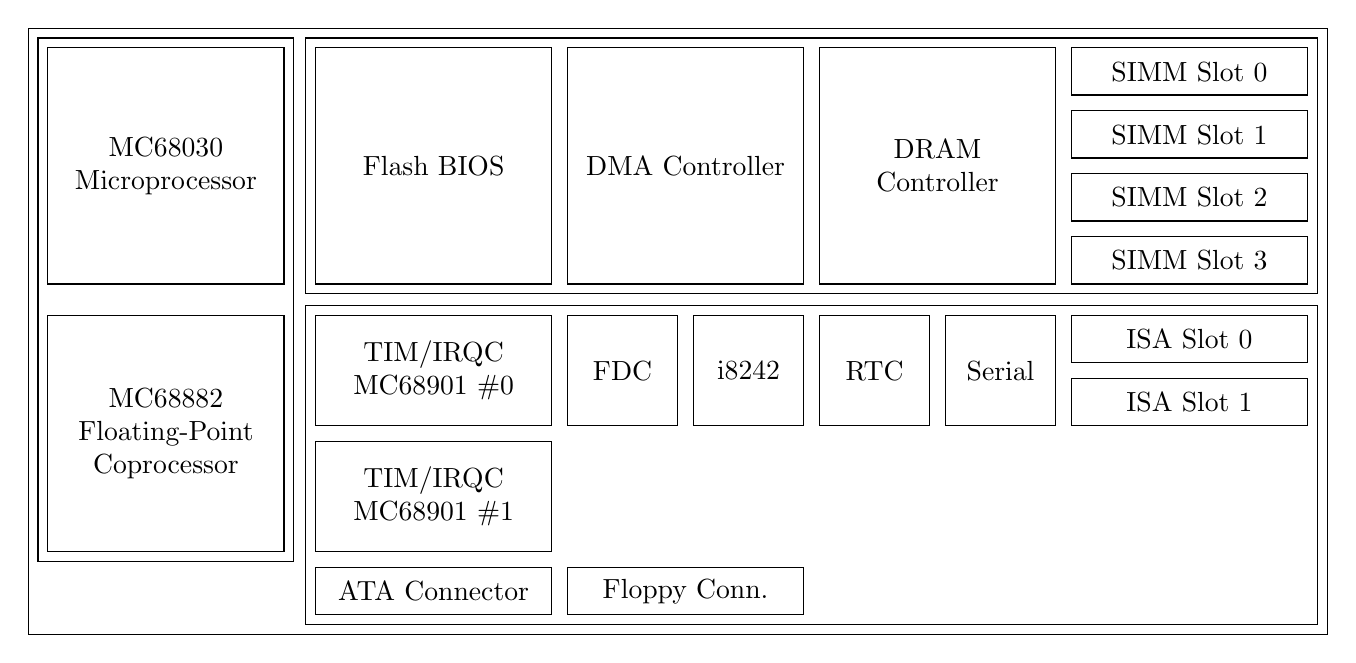
\begin{tikzpicture}[
    component_large/.style={rectangle, align=center, draw=black, thin, minimum width=3cm, minimum height=3cm},
    component/.style={rectangle, align=center, draw=black, thin, minimum width=3cm, minimum height=1.4cm},
    component_small/.style={rectangle, align=center, draw=black, thin, minimum width=1.4cm, minimum height=1.4cm},
    slot/.style={rectangle, align=center, draw=black, thin, minimum width=3cm, minimum height=6mm},
    conn/.style={rectangle, align=center, draw=black, thin, minimum width=3cm, minimum height=6mm},
    bus_unidir/.style={single arrow, draw=black, minimum width=0.5cm, single arrow head extend=2mm, minimum height=10mm},
    bus_bidir/.style={double arrow, draw=black, minimum width=0.5cm, double arrow head extend=2mm, minimum height=10mm},
    text/.style={},
]
    \node(cpu)[component_large] at (0, 0) {MC68030\\ Microprocessor};
    \node(fpu)[component_large] at (0, -34mm) {MC68882\\ Floating-Point\\ Coprocessor};
    \node(processor_group)[draw=black, fit={
        (cpu) (fpu)
    }]{};

    \node(bios)[component_large] at (34mm, 0) {Flash BIOS};
    \node(dmac)[component_large] at (66mm, 0) {DMA Controller};
    \node(dramc)[component_large] at (98mm, 0) {DRAM\\ Controller};
    \node(simm0)[slot] at (130mm, 12mm) {SIMM Slot 0};
    \node(simm1)[slot] at (130mm, 4mm) {SIMM Slot 1};
    \node(simm2)[slot] at (130mm, -4mm) {SIMM Slot 2};
    \node(simm3)[slot] at (130mm, -12mm) {SIMM Slot 3};
    \node(memory_group)[draw=black, fit={
        (bios) (dramc) (dmac) (simm0) (simm1) (simm2) (simm3)
    }]{};

    \node(irqc)[component] at (34mm, -26mm) {TIM/IRQC\\ MC68901 \#0};
    \node(irqc)[component] at (34mm, -42mm) {TIM/IRQC\\ MC68901 \#1};
    \node(fdc)[component_small] at (58mm, -26mm) {FDC};
    \node(i8242)[component_small] at (74mm, -26mm) {i8242};
    \node(rtc)[component_small] at (90mm, -26mm) {RTC};
    \node(duart)[component_small] at (106mm, -26mm) {Serial};
    \node(isa0)[slot] at (130mm, -22mm) {ISA Slot 0};
    \node(isa1)[slot] at (130mm, -30mm) {ISA Slot 1};
    \node(ata_conn)[conn] at (34mm, -54mm) {ATA Connector};
    \node(fdc_conn)[conn] at (66mm, -54mm) {Floppy Conn.};
    \node(peripheral_group)[draw=black, fit={
        (irqc) (isa0) (isa1) (ata_conn) (fdc_conn)
    }]{};

    %\node(local_data_bus)[bus_bidir, above right=-1cm and 3mm of cpu]{};
    %\node(local_address_bus)[bus_unidir, below right=-1cm and 3mm of cpu]{};
    \node(system)[draw=black, fit={
        (processor_group) (memory_group) (peripheral_group)
    }]{};
\end{tikzpicture}

\begin{flushleft}
    Contents in this chapter roughly explains about the entire architecture of
    the  Extensible HomeBrew Computer. The architecture of this system is
    designed to provide flexible operations, rich system functions, and large
    expansion capabilities. 
\end{flushleft}

\section{Features}

\begin{flushleft}
    The features and characteristics of the Extensible HomeBrew Computer
    (hereafter ``030EHBC'') are listed as follows:

    \begin{enumerate}
        \item Powered by a Motorola MC68030 microprocessor and a MC68882 coprocessor
        \begin{enumerate}
            \item 32-bit microprocessor up to 50 MHz of operation clock
            \item Integrated 256-byte data cache and 256-byte instruction cache
            \item Paged Memory-Management Unit (MMU) integrated for memory protection
            \item 7 levels of interrupt autovector
            \item A MC68882 floating-point coprocessor which accelerates real-number arithmetic is installable
        \end{enumerate}
        \item Configurable processor frequency up to 50MHz and two fixed clocks at 24MHz and at 14.61818MHz
        \item Four 72-pin SIMMs for DRAM capacity up to 64MiB
        \item Cache support with the SRAM capacity up to 4MiB of data space and 512kiB of tag space.
        \item The Cached DRAM Controller and the System Bus Controller implemented on FPGA:
        \begin{enumerate}
            \item The Cached DRAM Controller, CDC is a DRAM controller with a cache support. It also works as a 8-channel DMA controller.
            \item The System Bus Controller, SBC is a multifunctional bus controller which supports PEP, ISA, OPB, and Parallel ATA.
        \end{enumerate}
        \item Synchronous local bus transfer support by system controllers (CDC and SBC) in order to achieve fast operation cycles
        \item 8 DMA channels with detailed signal customizations
        \item Full support of IRQ signals driven by ISA bus devices
        \item 4 programmable timers
        \item Rich capabilities of peripheral buses and external devices:
        \begin{enumerate}
            \item Peripheral Expansion Port, PEP: 32-bit high-speed bus with multiplexed address and data
            \item Industry Standard Architecture, ISA: 8-bit or 16-bit ISA bus for IBM PC compatibility
            \item On-board Peripheral Bus, OPB: Simple 8-bit or 16-bit bus for integrated system peripherals
            \item Parallel AT-Attachment, PATA: ACS-4 compatible 16-bit bus for storage devices
            \item Inter-Integrated Circuit, I2C (IIC): Serial bus for system management and device recognization
            \item Serial Peripheral Interface, SPI: Serial bus for NVSRAM connection
            \item 1 floppy drive interface
            \item 1 USB host interface
            \item PS/2 keyboard and mouse interface
            \item 1 RS232 serial port
            \item 1 10Base-T 10Mbps ethernet port
            \item Speaker/Microphone/Line-in audio jack
        \end{enumerate}
        \item 5 expansion bus device connectors:
        \begin{enumerate}
            \item 3 sets of DIN-41612 3x32 and 3x10 connector for each PEP device
            \item 2 sets of a 36-pin and 62-pin card-edge socket for each ISA device
        \end{enumerate}
        \item Real-time clock and NVSRAM
        \item Coin cell battery backup for a RTC and a NVSRAM
        \item Two 4MiB flash memories storing firmware code and data
        \item A dual-channel step-down buck converter providing adjustable voltage supplies to processors and system controllers.
        \item A power monitor supervising voltage and current of each power supply rails
        \item A System Master Controller implemented on ATMega32 controls switches, a buzzer, reset signals, etc.
        \item A 24-pin ATX power supply connector for power inputs
    \end{enumerate}
\end{flushleft}

\chapter{Processor \& Coprocessor}
\section{The Main Processor}
\section{The Coprocessor}
\chapter{Memory Subsystem}
\section{System Memory Types}
\section{Memory Map}
\subsection{Supervisor Address Space}
\subsection{User Address Space}
\section{The Main Dynamic RAM Module}
\section{The Cache RAM Module}
\section{Memory-Mapped I/O}
\section{Direct Memory Access}
\chapter{System Controllers}
\section{Cached DRAM Controller}
\section{System Bus Controller}
\section{System Master Controller}
\chapter{System Bus}
\section{Local Bus}
\section{PEP Bus}
\section{ISA Bus}
\section{Parallel ATA Bus}
\chapter{Prepheral Expansion Port}
\chapter{On-Board Peripherals}
\chapter{External Peripherals}
\chapter{Power Supply}
\chapter{Debugging Interfaces}
\chapter{Firmware}
\chapter{System Initialization}

\end{document}
